
\subsubsection{Final trigger strategy}

Based on the studies and efficiency measurements detailed in the rest of this section, the following trigger strategy is used in the analysis:

\begin{itemize}

\item If $\met$ < 250 GeV, only an \texttt{OR} combination of the following di-lepton triggers is used: \\HLT\_2e12\_lhloose\_L12EM10VH, HLT\_e17\_lhloose\_mu14, HLT\_mu18\_mu8noL1.

\item If $\met$ > 250 GeV, an \texttt{OR} between the di-lepton triggers and \texttt{HLT\_xe70} is used.

\end{itemize}

Trigger matching is applied as follows:
\begin{itemize}
\item only signal leptons with $\pt>20$~Gev are considered
\item for technical reasons, matching to muon triggers is performed only on the corresponding level-1 item (L1\_MU10 and L1\_MU15)
\item trigger matching for HLT\_mu18\_mu8noL1 is performed only on the mu18 leg; however, the presence of another signal muon in the event is required. 
\end{itemize}

\subsubsection{Detailed trigger studies (DC14, MC15)}

The trigger strategy for the analysis in Run-2 is similar to the one used in the Run-1 version. There, a combination of \met, single-lepton and di-lepton triggers was used for the selection of events in the signal regions as well as for background estimations. The triggers were checked consecutively starting with the \met\ trigger, followed by the single-lepton trigger and the di-lepton triggers, until one of the triggers is passed by the event. Offline cuts on the missing energy and the \pt\ of the triggered objects were applied to ensure to be on the efficiency plateau of the corresponding trigger.

For Run-2, the triggers to be considered are single-lepton, di-lepton triggers and a $\met$ trigger. The lepton trigger menu includes di-lepton triggers selecting same-flavour and mixed-flavour lepton events. Some single-lepton triggers have additional requirements on the isolation of the triggered lepton. The following triggers have been regarded as important for this analysis and were used for further studies on performance and efficiency:

\begin{itemize}
\item Single-lepton triggers: \texttt{HLT\_mu26, HLT\_mu50, HLT\_mu24\_imedium, HLT\_mu26\_imedium}, 

\texttt{HLT\_e20\_medium, HLT\_e60\_medium, HLT\_e24\_tight\_iloose, HLT\_e26\_tight\_iloose}

\item Di-lepton triggers: \texttt{HLT\_2e12\_loose\_L12EM10VH, HLT\_2e12\_lhloose\_L12EM10VH}

\texttt{HLT\_e17\_loose\_mu14, HLT\_e17\_lhloose\_mu14, HLT\_mu18\_mu8noL1}

\item \met\ trigger: \texttt{HLT\_xe100}

\end{itemize}

Note that the low-$\pt$ single-lepton triggers which would be run un-prescaled in 2015 contain requirements on the lepton isolation ({\tt iloose}, {\tt imedium}) 
and/or more stringent electron identification requirements ({\tt medium}) than those used in the baseline lepton definition. 
Therefore we can't rely on these chains to select the sample of event to be used for fake-lepton background estimation, 
although they might still be useful for signal region selection.

The performance of these triggers has been investigated by running the analysis on dedicated Monte Carlo samples. 
For each object triggered, an offline cut on the object \pt\ or the \met\ is applied to ensure the full efficiency of the trigger in the selected event. 
We ensure that the tested trigger was activated by one of the signal leptons found in the analysis, 
by requiring a geometrical $\Delta R$ matching between these signal leptons 
and the leptons reconstructed by the online version of the software, responsible for the trigger decision. 


\paragraph{Monte Carlo samples and software framework}

The analysis code was setup with the \texttt{AnalysisBase} framework (2.3.8 branch for rel.20 ATLAS software). 
The object selection was done by using the \texttt{SUSYTools-00-06-03} package 
which the recommended selections of signal and baseline objects at the time of the study. 

The Monte Carlo samples used for these studies are validation samples produced with the 20.1.4.3 MC15 ATLAS software release. 
%The samples used for this study do not contain pile-up simulation. 

\begin{itemize}

\item $t \bar{t}$ sample: 

\texttt{valid3.110401.PowhegPythia\_P2012\_ttbar\_nonallhad.recon.AOD.e3099\_s2578\_r6540}

\item $Z \rightarrow \mu \mu$ sample:  

\texttt{valid3.167826.Sherpa\_CT10\_ZmumuMassiveCBPt280\_500\_CVetoBVeto.recon.AOD.e3099\_s2578\_r6540}

\item $Z \rightarrow e e$ sample: 

\texttt{valid3.147406.PowhegPythia8\_AZNLO\_Zee.recon.AOD.e3099\_s2578\_r6540}

\end{itemize}

\paragraph{Total event yields}

The total event yields for the test Monte Carlo samples and different trigger configurations were investigated in order to understand the gain of the several trigger types and their combinations. The yields are measured in a $t \bar{t}$ Monte Carlo sample and for different trigger applications applied. The three configuration tested were:
\begin{enumerate}
\item Applying only di-lepton triggers ({\tt HLT\_2e12\_loose\_L12EM10VH}, {\tt HLT\_2e12\_lhloose\_L12EM10VH}, {\tt HLT\_mu18\_mu8noL1}, {\tt HLT\_e17\_loose\_mu14}, {\tt HLT\_e17\_lhloose\_mu14})
\item Applying a logical \texttt{OR} between di-lepton triggers and the \met trigger ({\tt HLT\_xe100})
\item Applying a logical \texttt{OR} between di-lepton, \met, and single-lepton triggers without explicit isolation requirements ({\tt HLT\_e60\_lhmedium}, {\tt HLT\_mu50})
\end{enumerate}

The results are shown in Figure~\ref{fig:triggerYields}, separately  for events with $\met < 200$ GeV and 	$\met > 200$ GeV. While for the low-\met events, the single-lepton triggers induce a enhancement on the yields of about 1.5\%, the measurement for high-\met events shows only a negligible gain by adding single-lepton triggers to the configuration. The most significant increase is induced by adding the \met trigger to the di-lepton trigger chain for events with $\met > 200$ GeV, with a 6\% increase in the event yields. 
Therefore, the logical \texttt{OR} of di-lepton and $\met$ triggers will be used in the analysis.
For simplicity and due to the small improvement they could provide, single-lepton triggers will not be used in the following. 

\begin{figure}[htb!]
\centering
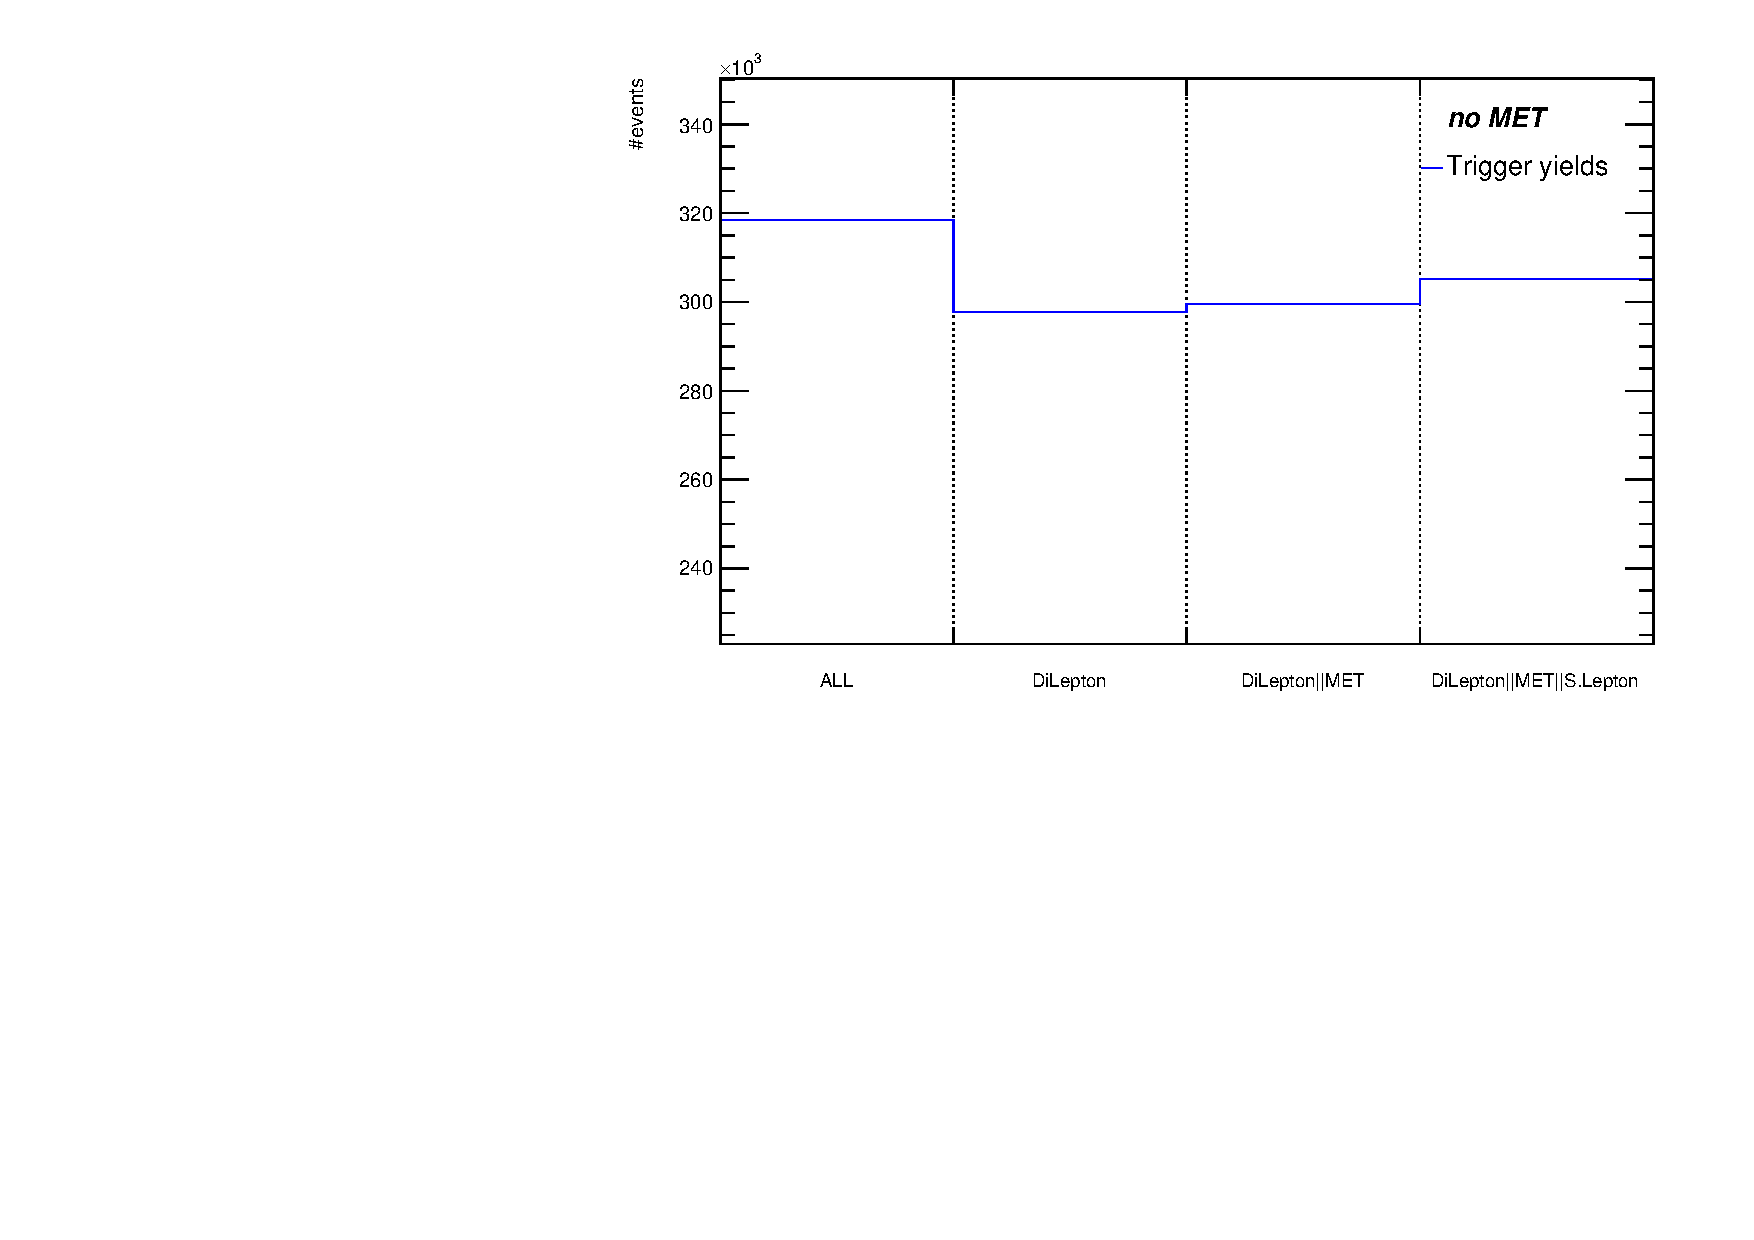
\includegraphics[width=0.49\textwidth]{TRIGGER/Yields_noMet.pdf}
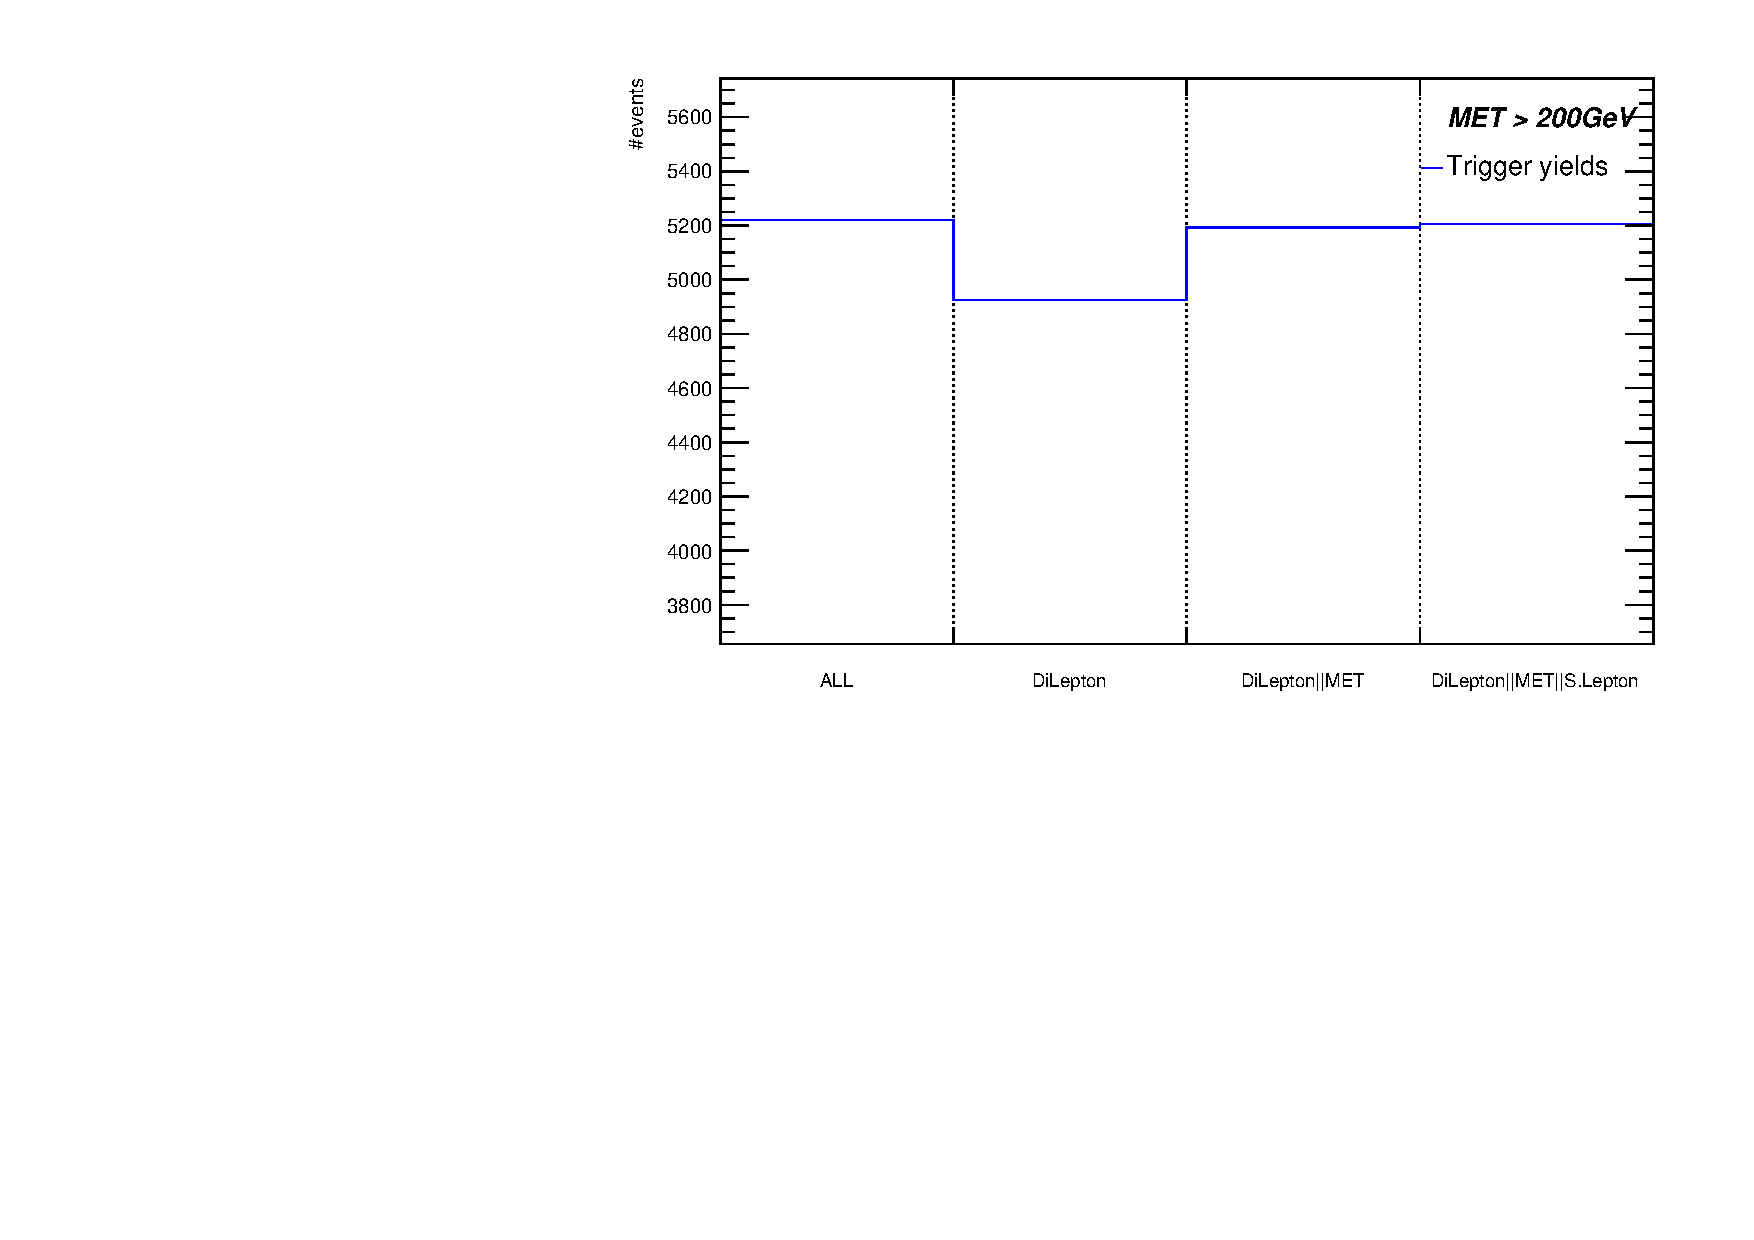
\includegraphics[width=0.49\textwidth]{TRIGGER/Yields_Met.pdf}
\caption{Total events yields of the $t\bar{t}$ sample for several trigger configurations. The yields are measured for events with $\met < 200$ GeV (left) and $\met > 200$ GeV (right) independently.}
\label{fig:triggerYields}
\end{figure}

\paragraph{Efficiencies}

The trigger efficiency in Monte Carlo can be obtained by dividing the number of triggered events by the total number of events. The generic cleaning cuts are applied in both cases. 


The efficiencies have been calculated separately for single-lepton, di-lepton triggers and for \met\ triggers. 
The results for some examples are shown in Fig.~\ref{fig:triggerEff} for di-lepton and \met\ triggers. 
%Further efficiency plots can be found in Appendix~\ref{app_trigger}. 
The turn-on curve for the \met trigger shows the expected evolution. 
The efficiency plateau is reached for $\met > 150-200$ GeV. At the trigger plateau, the efficiency is reaching $>99\%$. 
The combination of di-lepton and missing energy trigger shows an efficiency of $>90\%$ for di-muon events.

\begin{figure}[htb!]
\centering
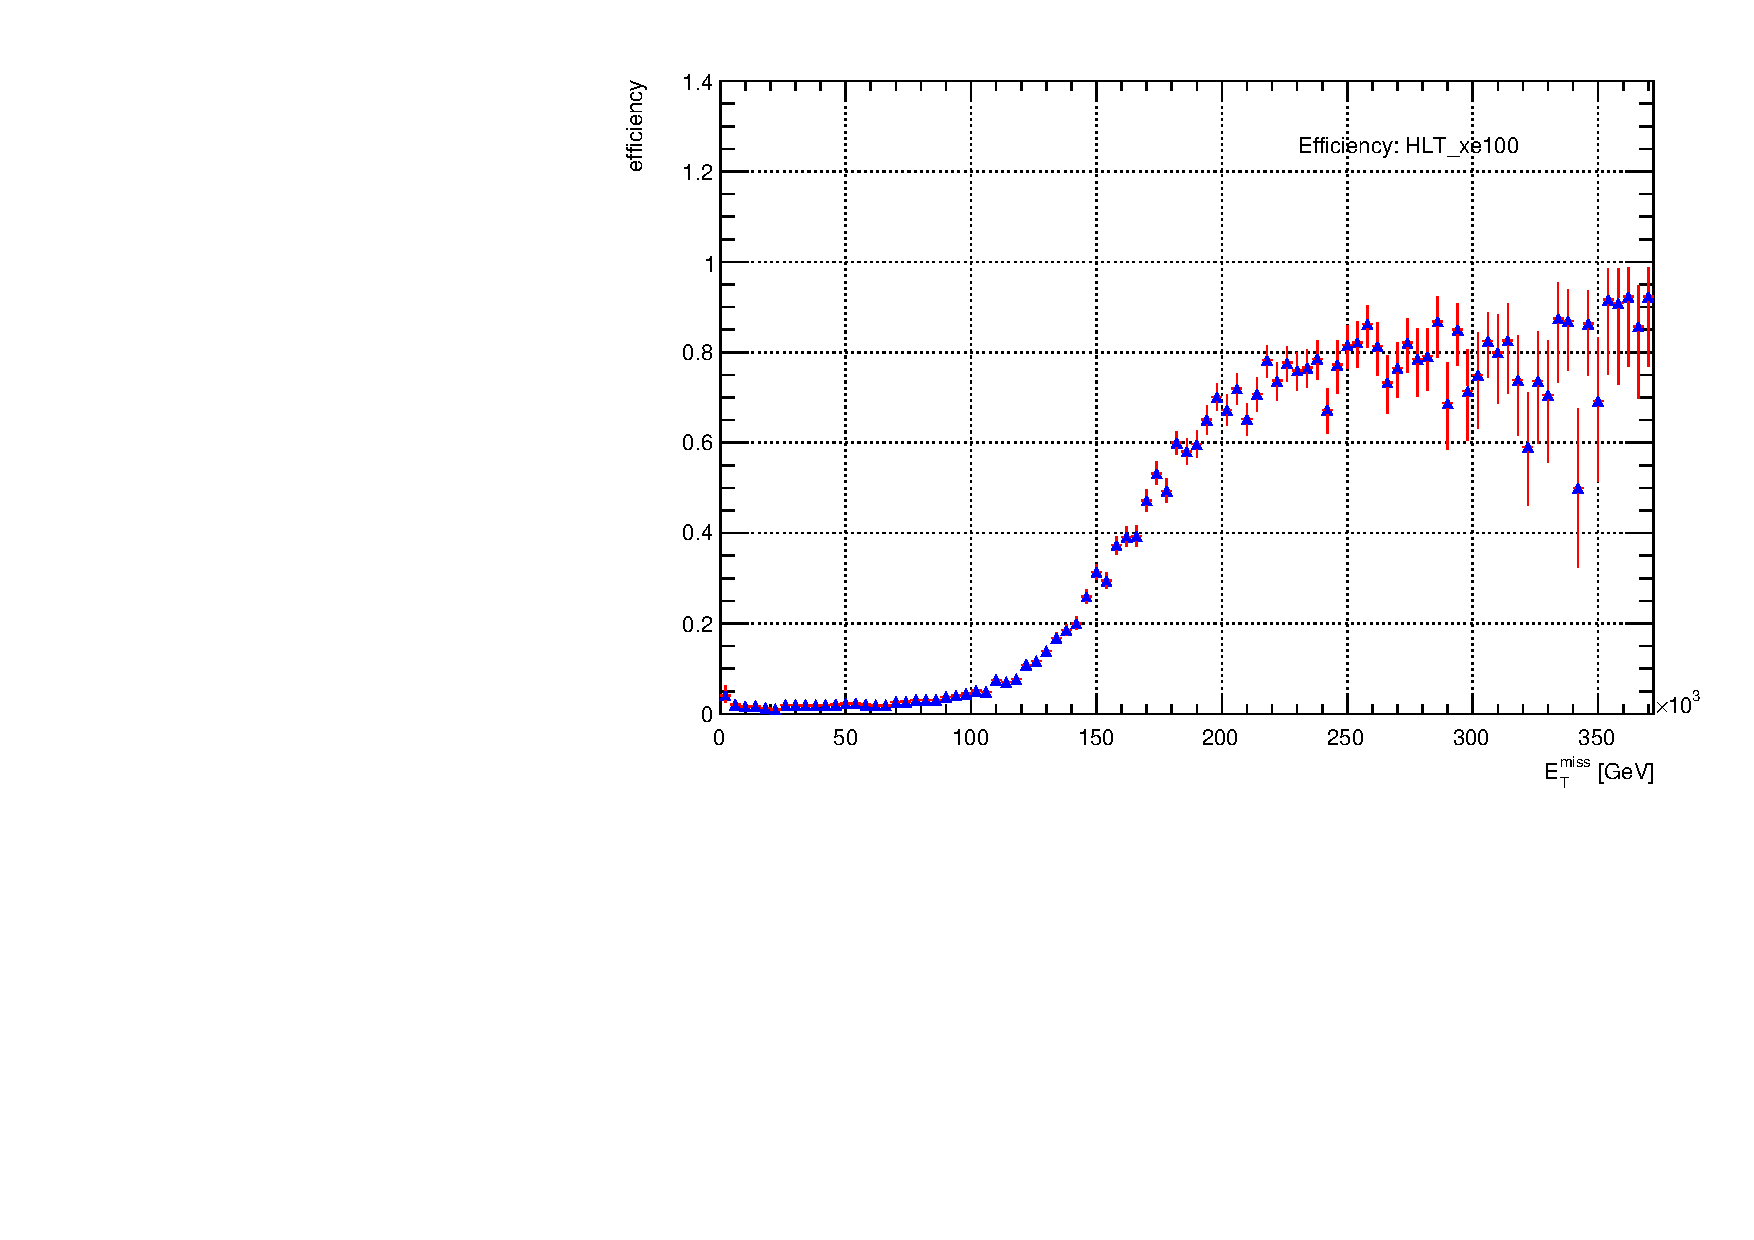
\includegraphics[width=0.49\textwidth]{TRIGGER/Eff_HLT_xe100.pdf}
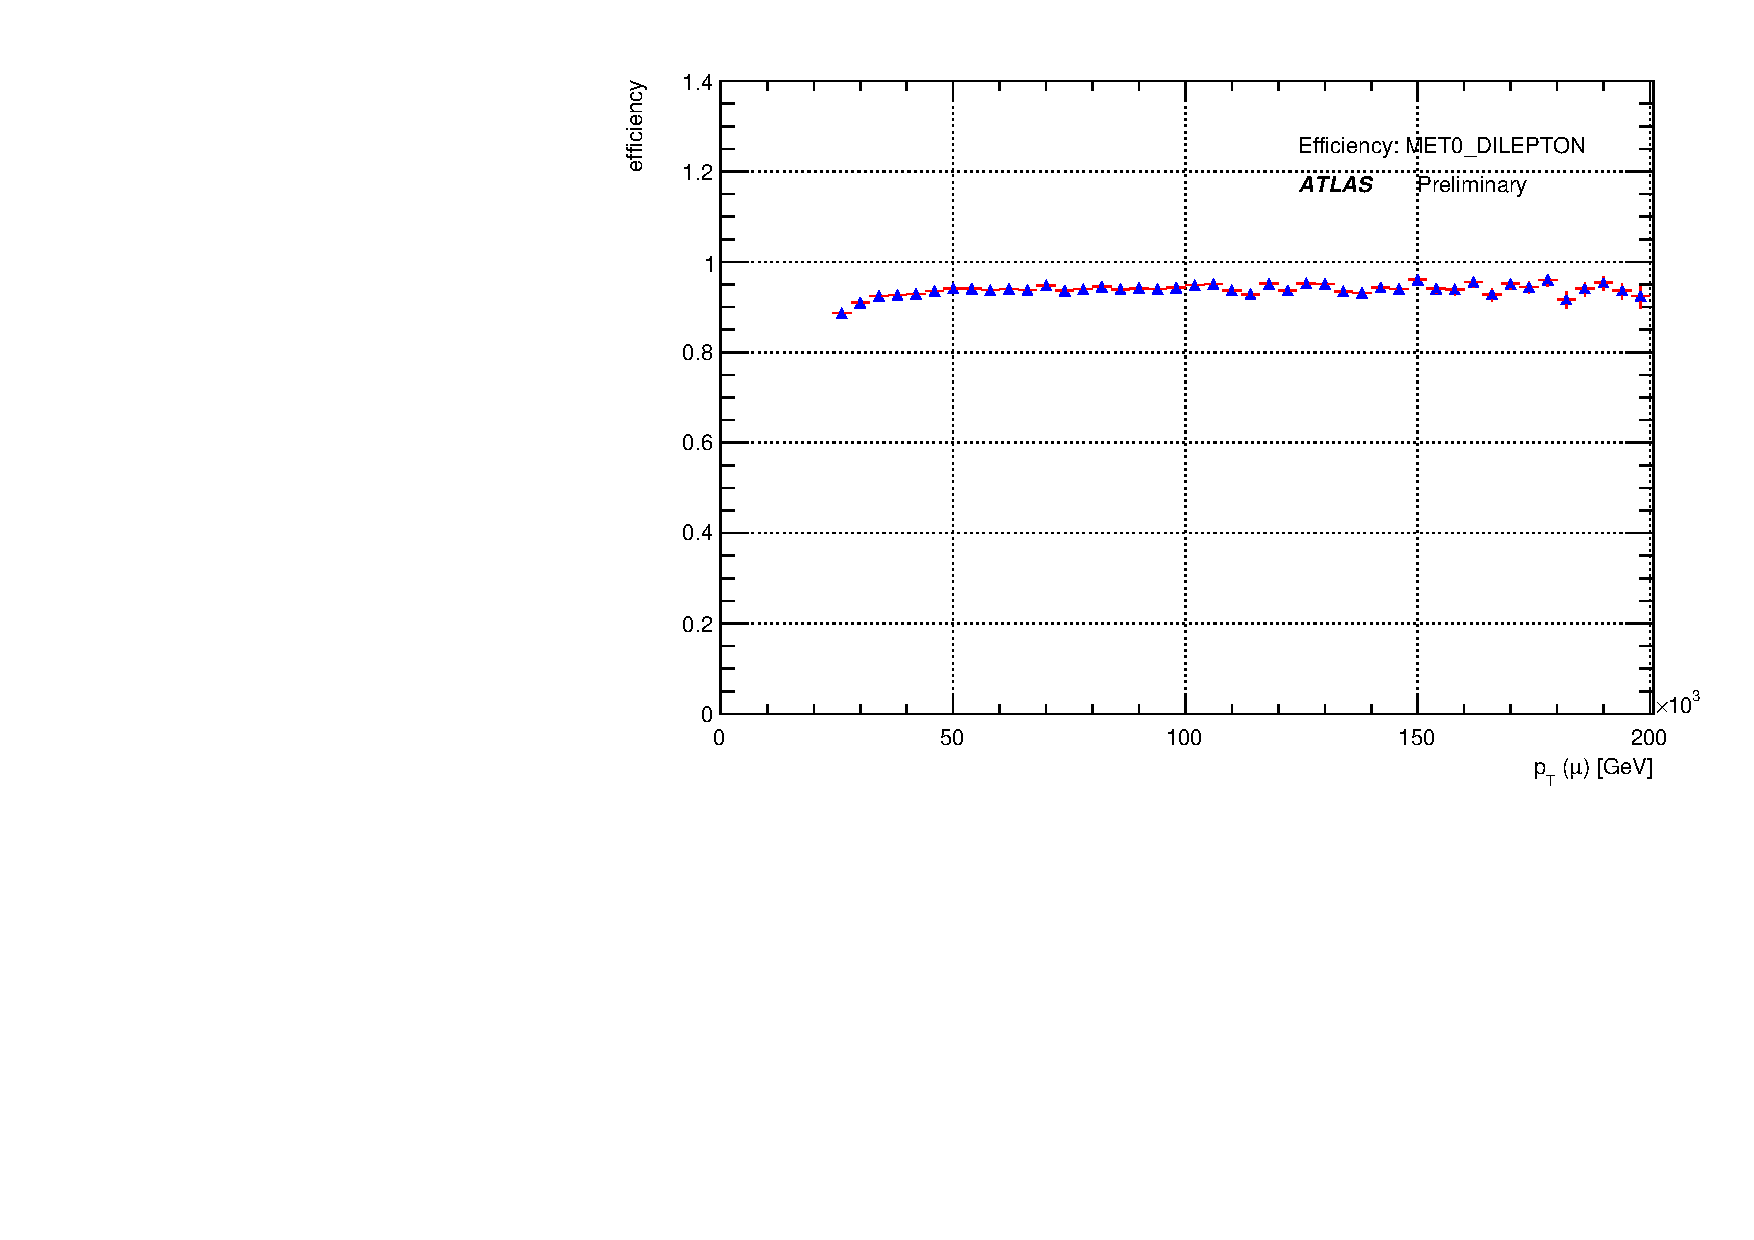
\includegraphics[width=0.49\textwidth]{TRIGGER/Eff_MET0_DILEPTON_1stMu.pdf}
\caption{Trigger efficiencies for \texttt{HLT\_xe100} (left) versus the missing energy and for the combination of di-lepton and \met-triggers (right) versus the \pt of the leading trigered muon.}
\label{fig:triggerEff}
\end{figure}



\paragraph{Choice of $\met$ trigger}

During the review of this analysis, it was pointed out that \texttt{xe\_70} trigger will be unprescaled during the 2015. 
Figure~\ref{fig:triggerEff_xe70_main} shows the turn-on curves of this trigger item for different requirements in the jet multiplicity,
and compared with \texttt{xe\_80} items. In all cases, the plateau of these trigger is reached at a $\met$ value of 250 GeV. More details can be found in App.~\ref{ap:met_update}.

\begin{figure}[htb!]
\centering
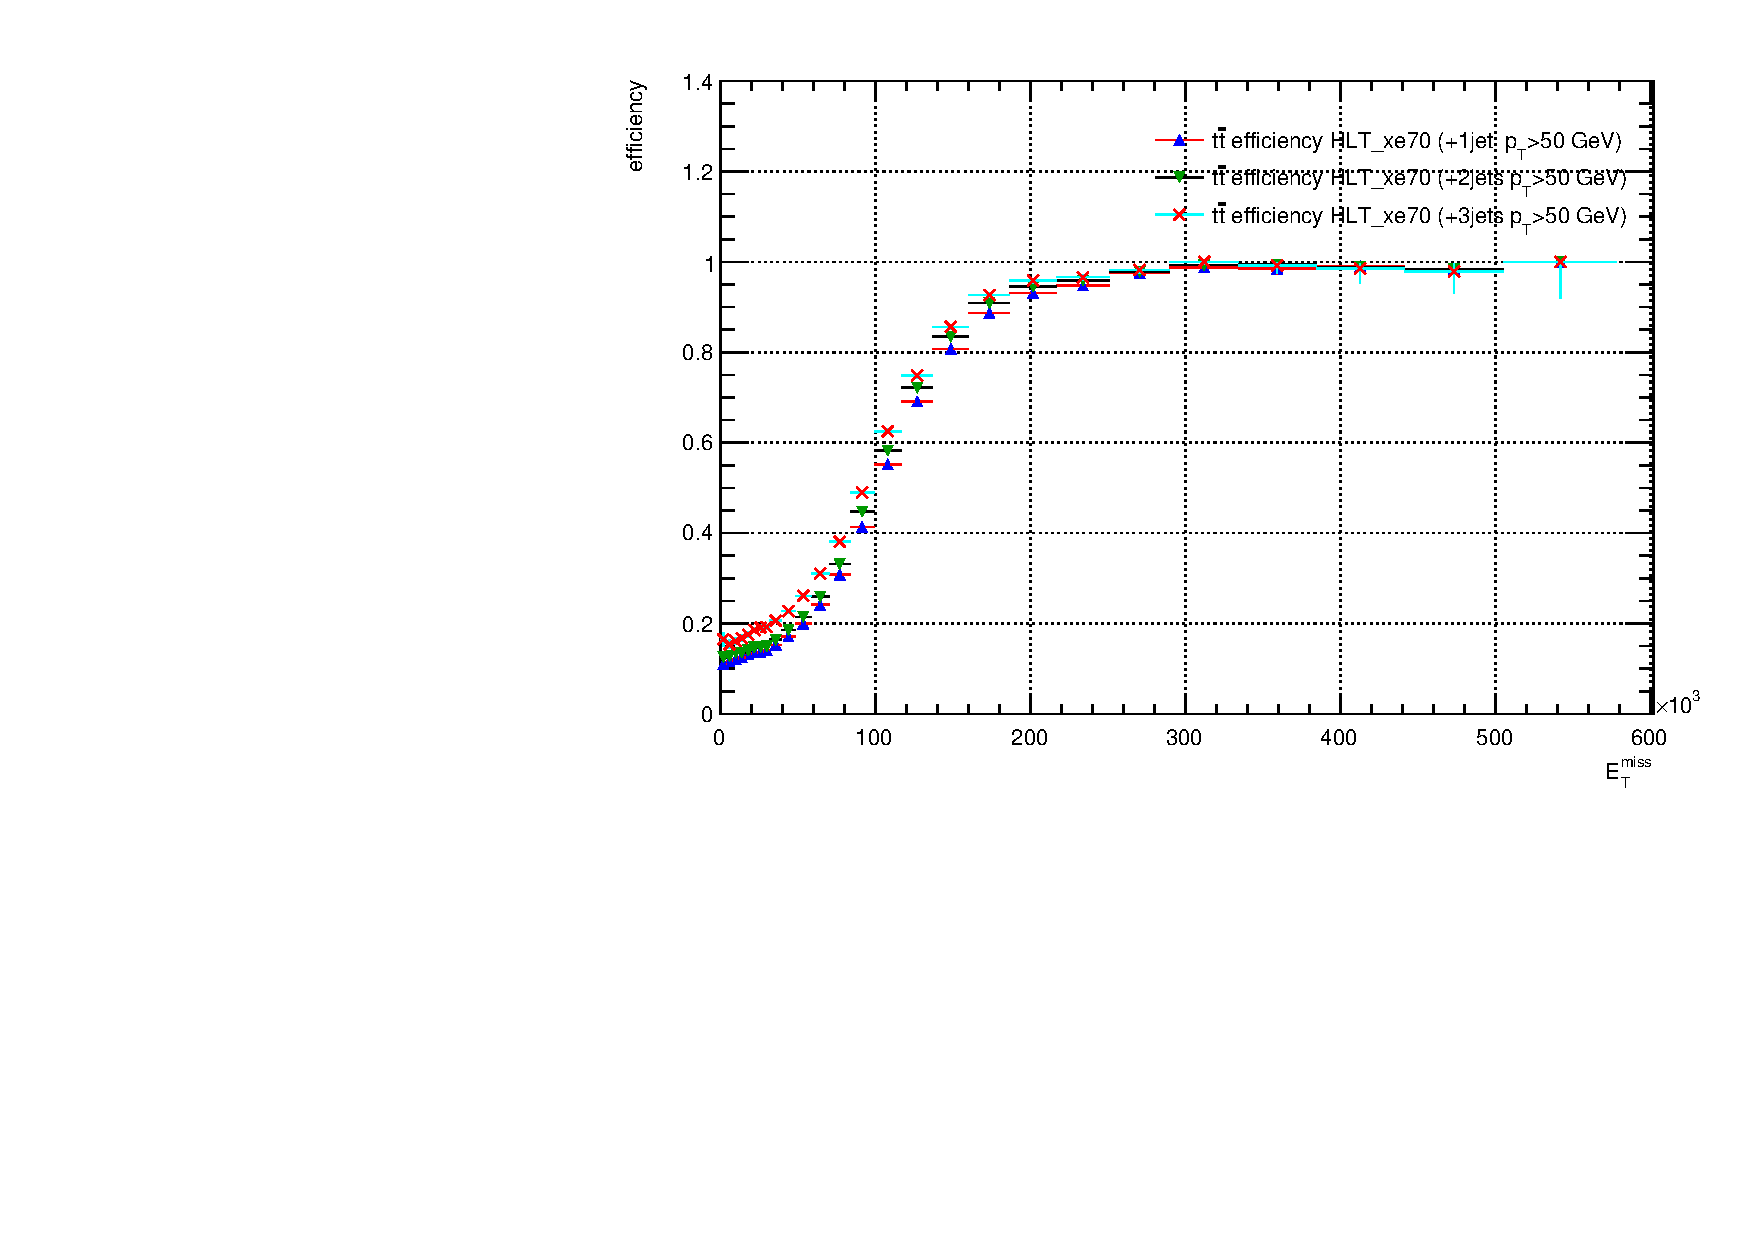
\includegraphics[width=0.50\textwidth]{TRIGGER/Eff_HLT_xe70_jets_MC.pdf}
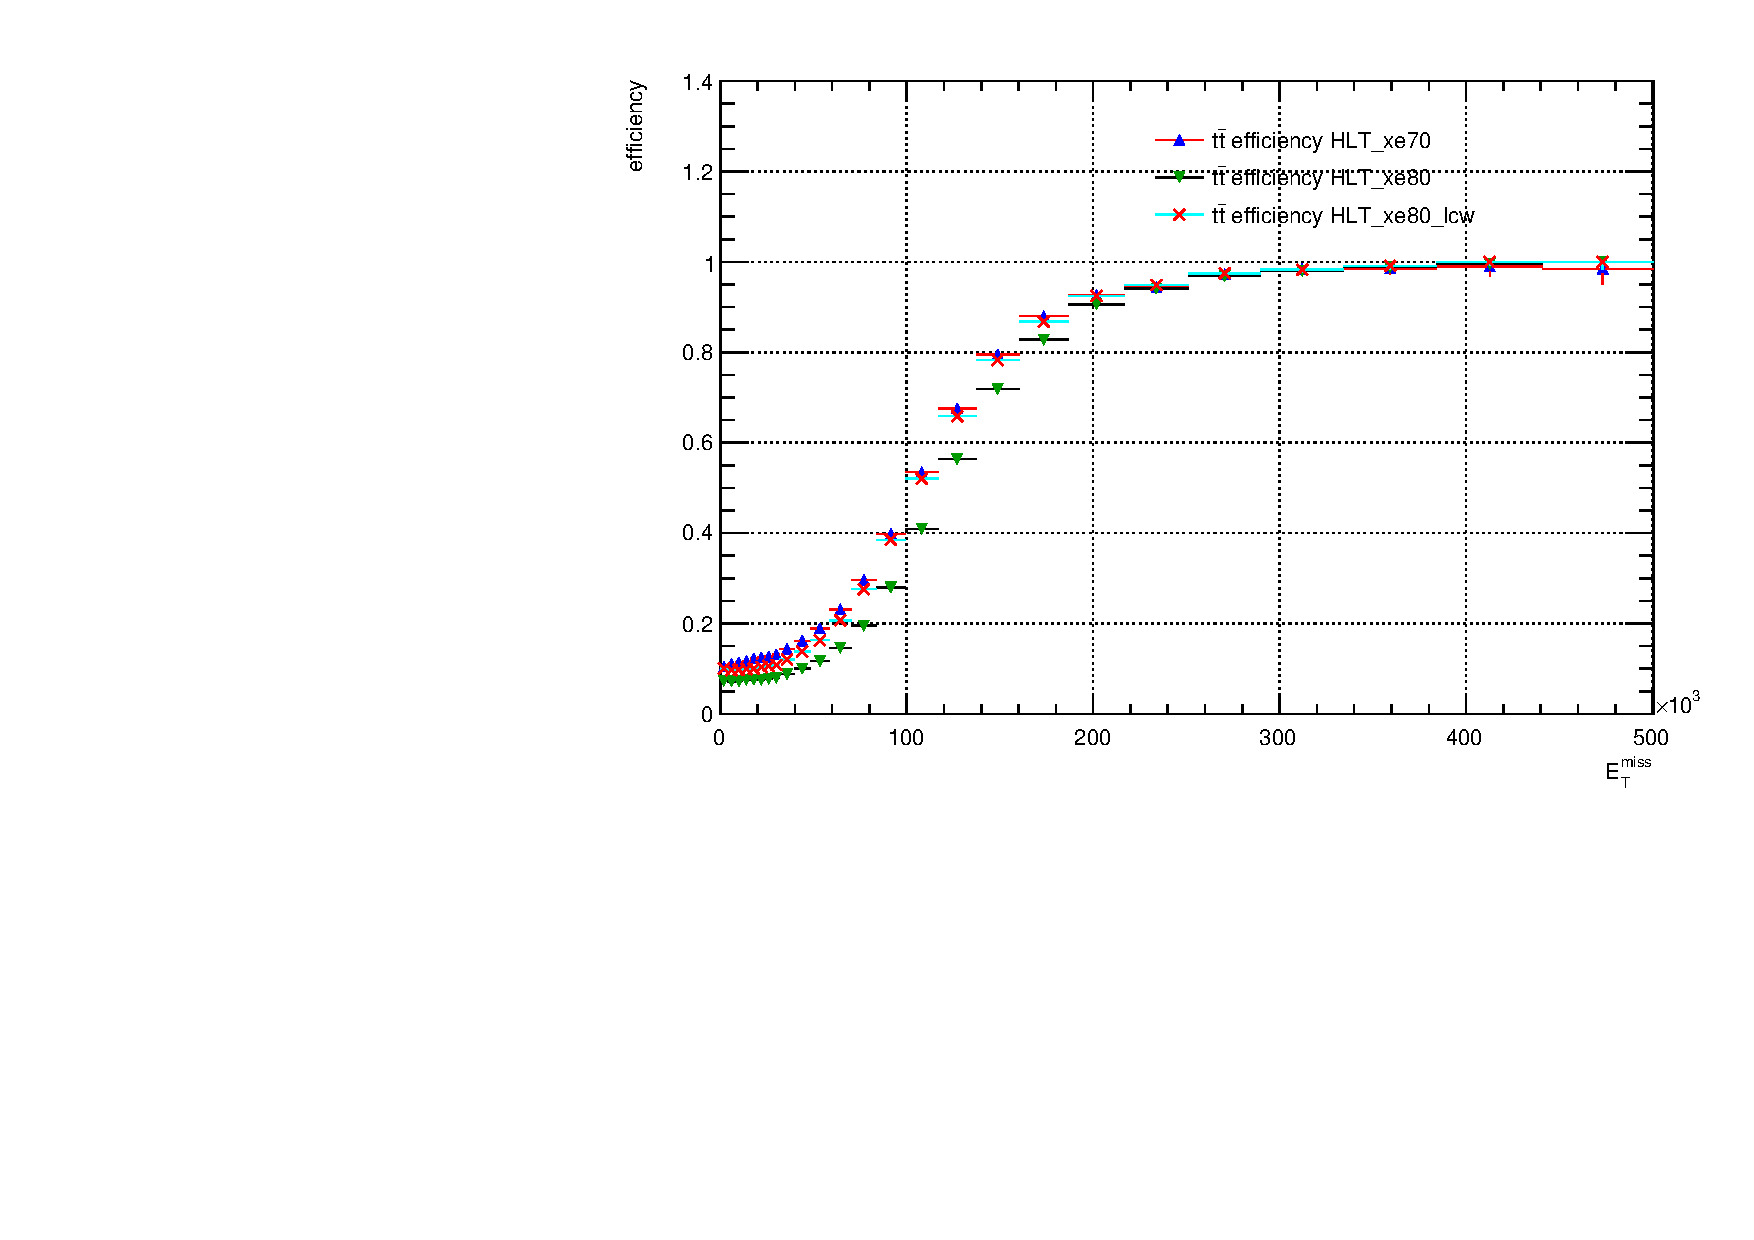
\includegraphics[width=0.49\textwidth]{TRIGGER/Eff_HLT_xe70_HLT_xe80.pdf}
\caption{Trigger efficiencies in data for \texttt{HLT\_xe70} (left) and \texttt{HLT\_xe80}, \texttt{HLT\_xe80\_tc\_lcw} (right) versus $\met$. The different curves show the efficiency for events containing a di-lepton pair.}
 \label{fig:triggerEff_xe70_main}
\end{figure}


Based on these studies and efficiency measurements, a preliminary decision for the trigger selection has been made.

\begin{itemize}

\item If $\met$ < 250 GeV, only an \texttt{OR} combination of di-lepton triggers is used. 

\item If $\met$ > 250 GeV, an \texttt{OR} between the di-lepton triggers and \texttt{HLT\_xe70} is used.

\end{itemize}